%!TEX root = ../data-imputation.tex
\section{Results}
\label{sec:results}

\felix{This entire section is the most important section of this paper. It's difficult to work on / comment on this section in its current shape. The content is lacking and the text needs some serious proofreading.}

\felix{why did we choose the rank in the first place? it's important to motivate that decision here by pointing to the heterogeneity of the results which we want to aggregate over}
The \textit{imputation rank} is the rank of the six imputers imputation performance on a single dataset-column combination. The values therefore lie within the interval [1, 6]. For numerical columns it is based on RMSE where lower is better. And for categorical columns it is based on the F1 macro score where higher is better. $n$ imputers with equal performance are assigned the same rank $r$ and the next best imputer gets the rank $r+n$.


\begin{figure}\centering
    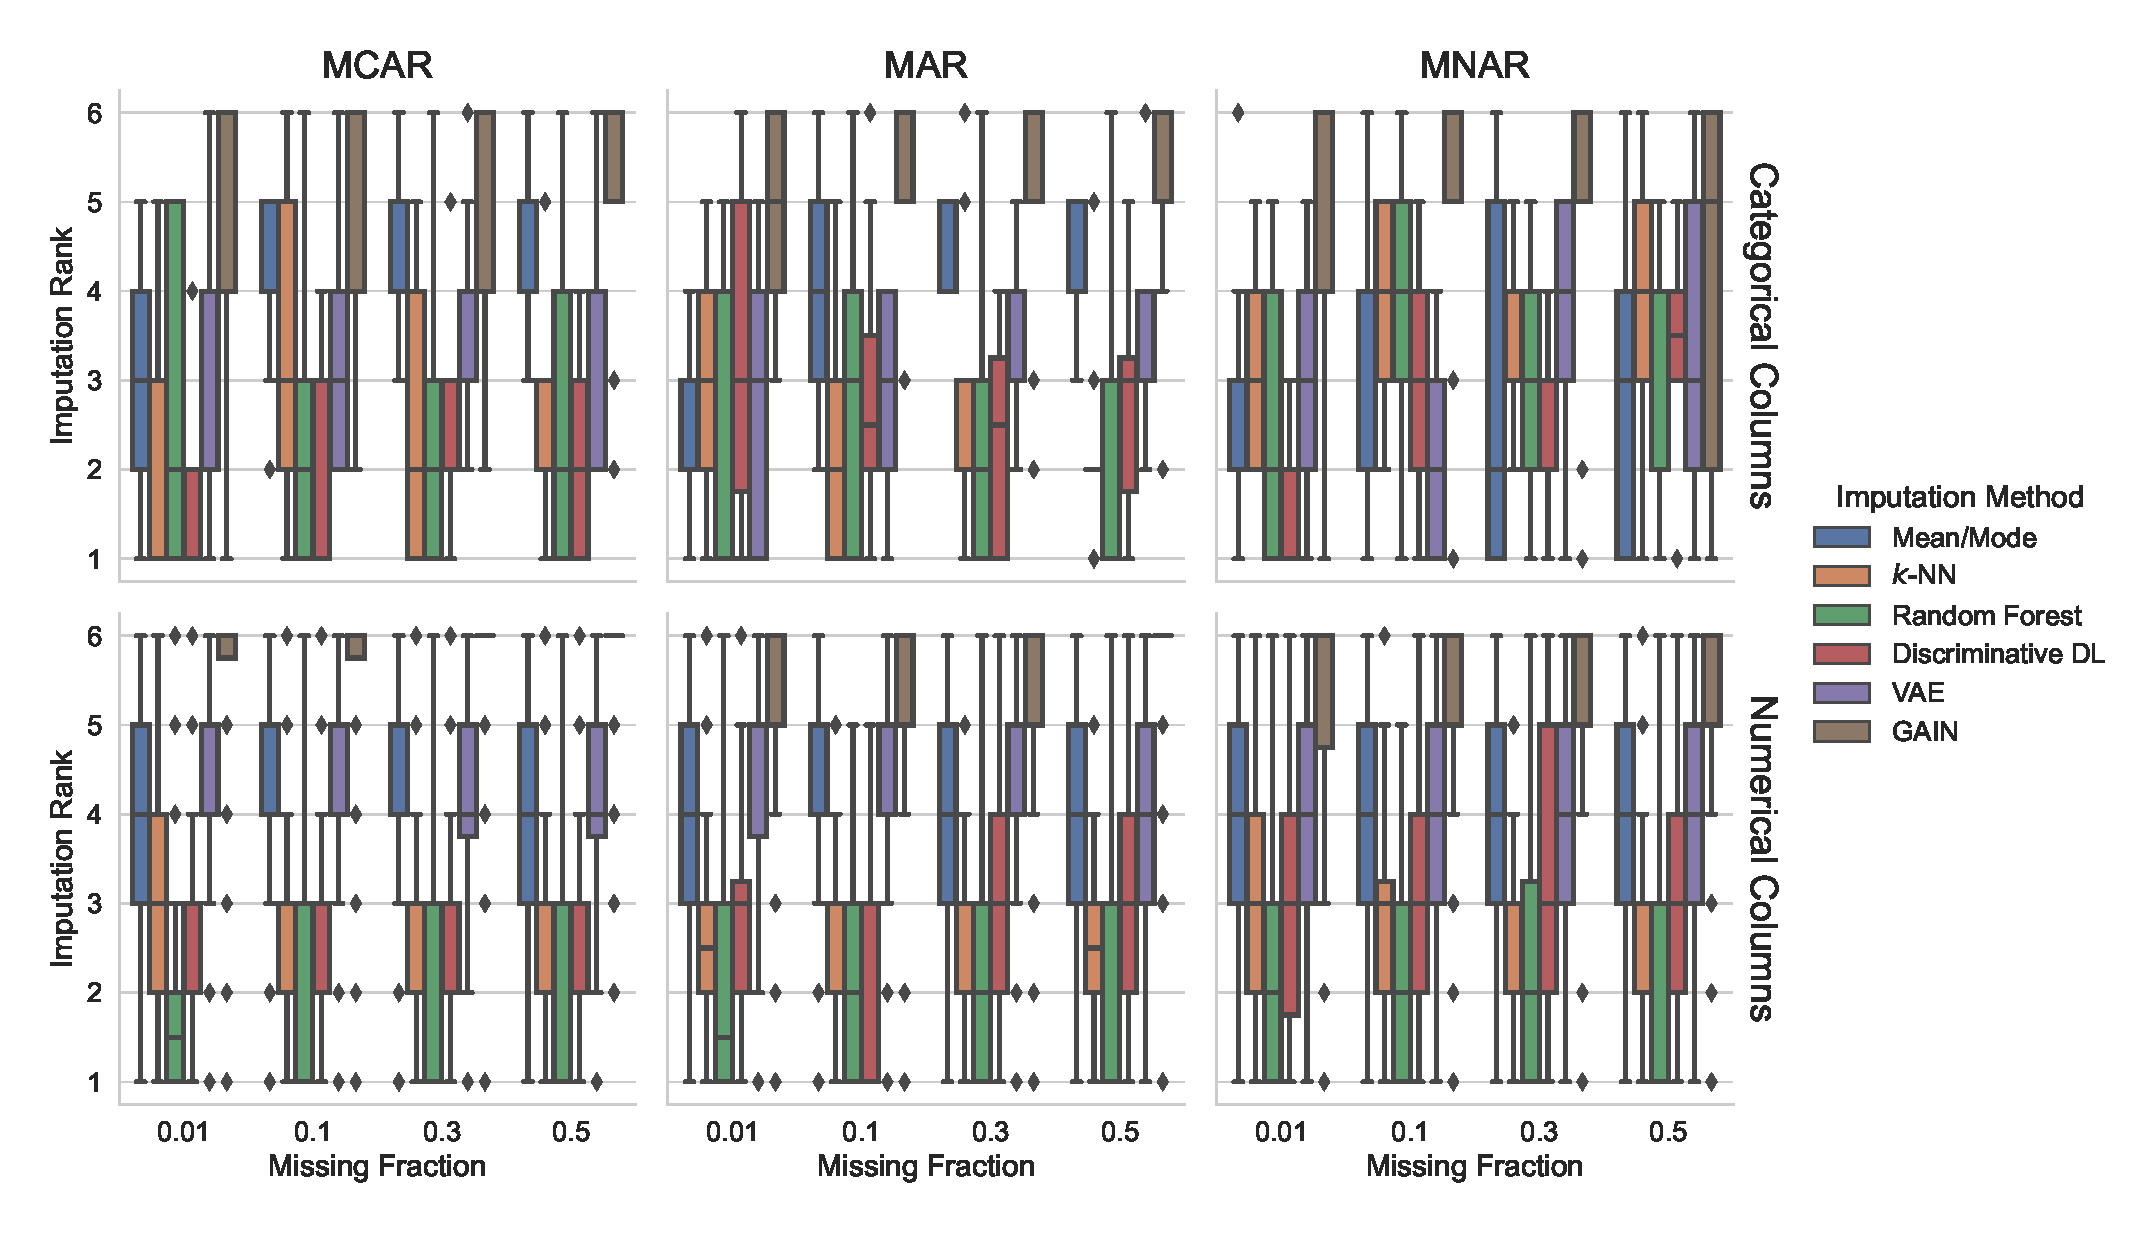
\includegraphics[width=1\columnwidth]{fully_observed_impute_rank_boxplot.eps}
    \caption[Scenario 1 Imputation Ranks]{In this figure, we visualize the results of \textit{Experiment 1} (imputation quality) in \textit{Scenario 1}. The imputation rank is plotted against the missingness fraction. The plot is divided into six sub-plots, with three columns determined by the missingness type, ordered by task difficulty from easiest to hardest (MCAR, MAR, MNAR). In the first row of sub-plots we depict results of regression tasks, whereas the second row contains classification results. Within a single sub-plot, each box represents the distibution of ranks of a single imputer over all corresponding datasets/columns.}\label{fig:fully_observed_impute_rank_boxplot}
\end{figure}

In Figure \ref{fig:fully_observed_impute_rank_boxplot} we observe that the \textit{forest imputer} performs best. It is the only one with 50\% of values among the first two ranks. In the MCAR and MNAR setting, another 25\% of values are on the third rank, whereas in the MNAR setting this spreads until rank four. However, the whiskery indicate that there are also some results ranging on the middle and even last ranks. (TODO rational for that?)
TODO

\begin{figure}\centering
    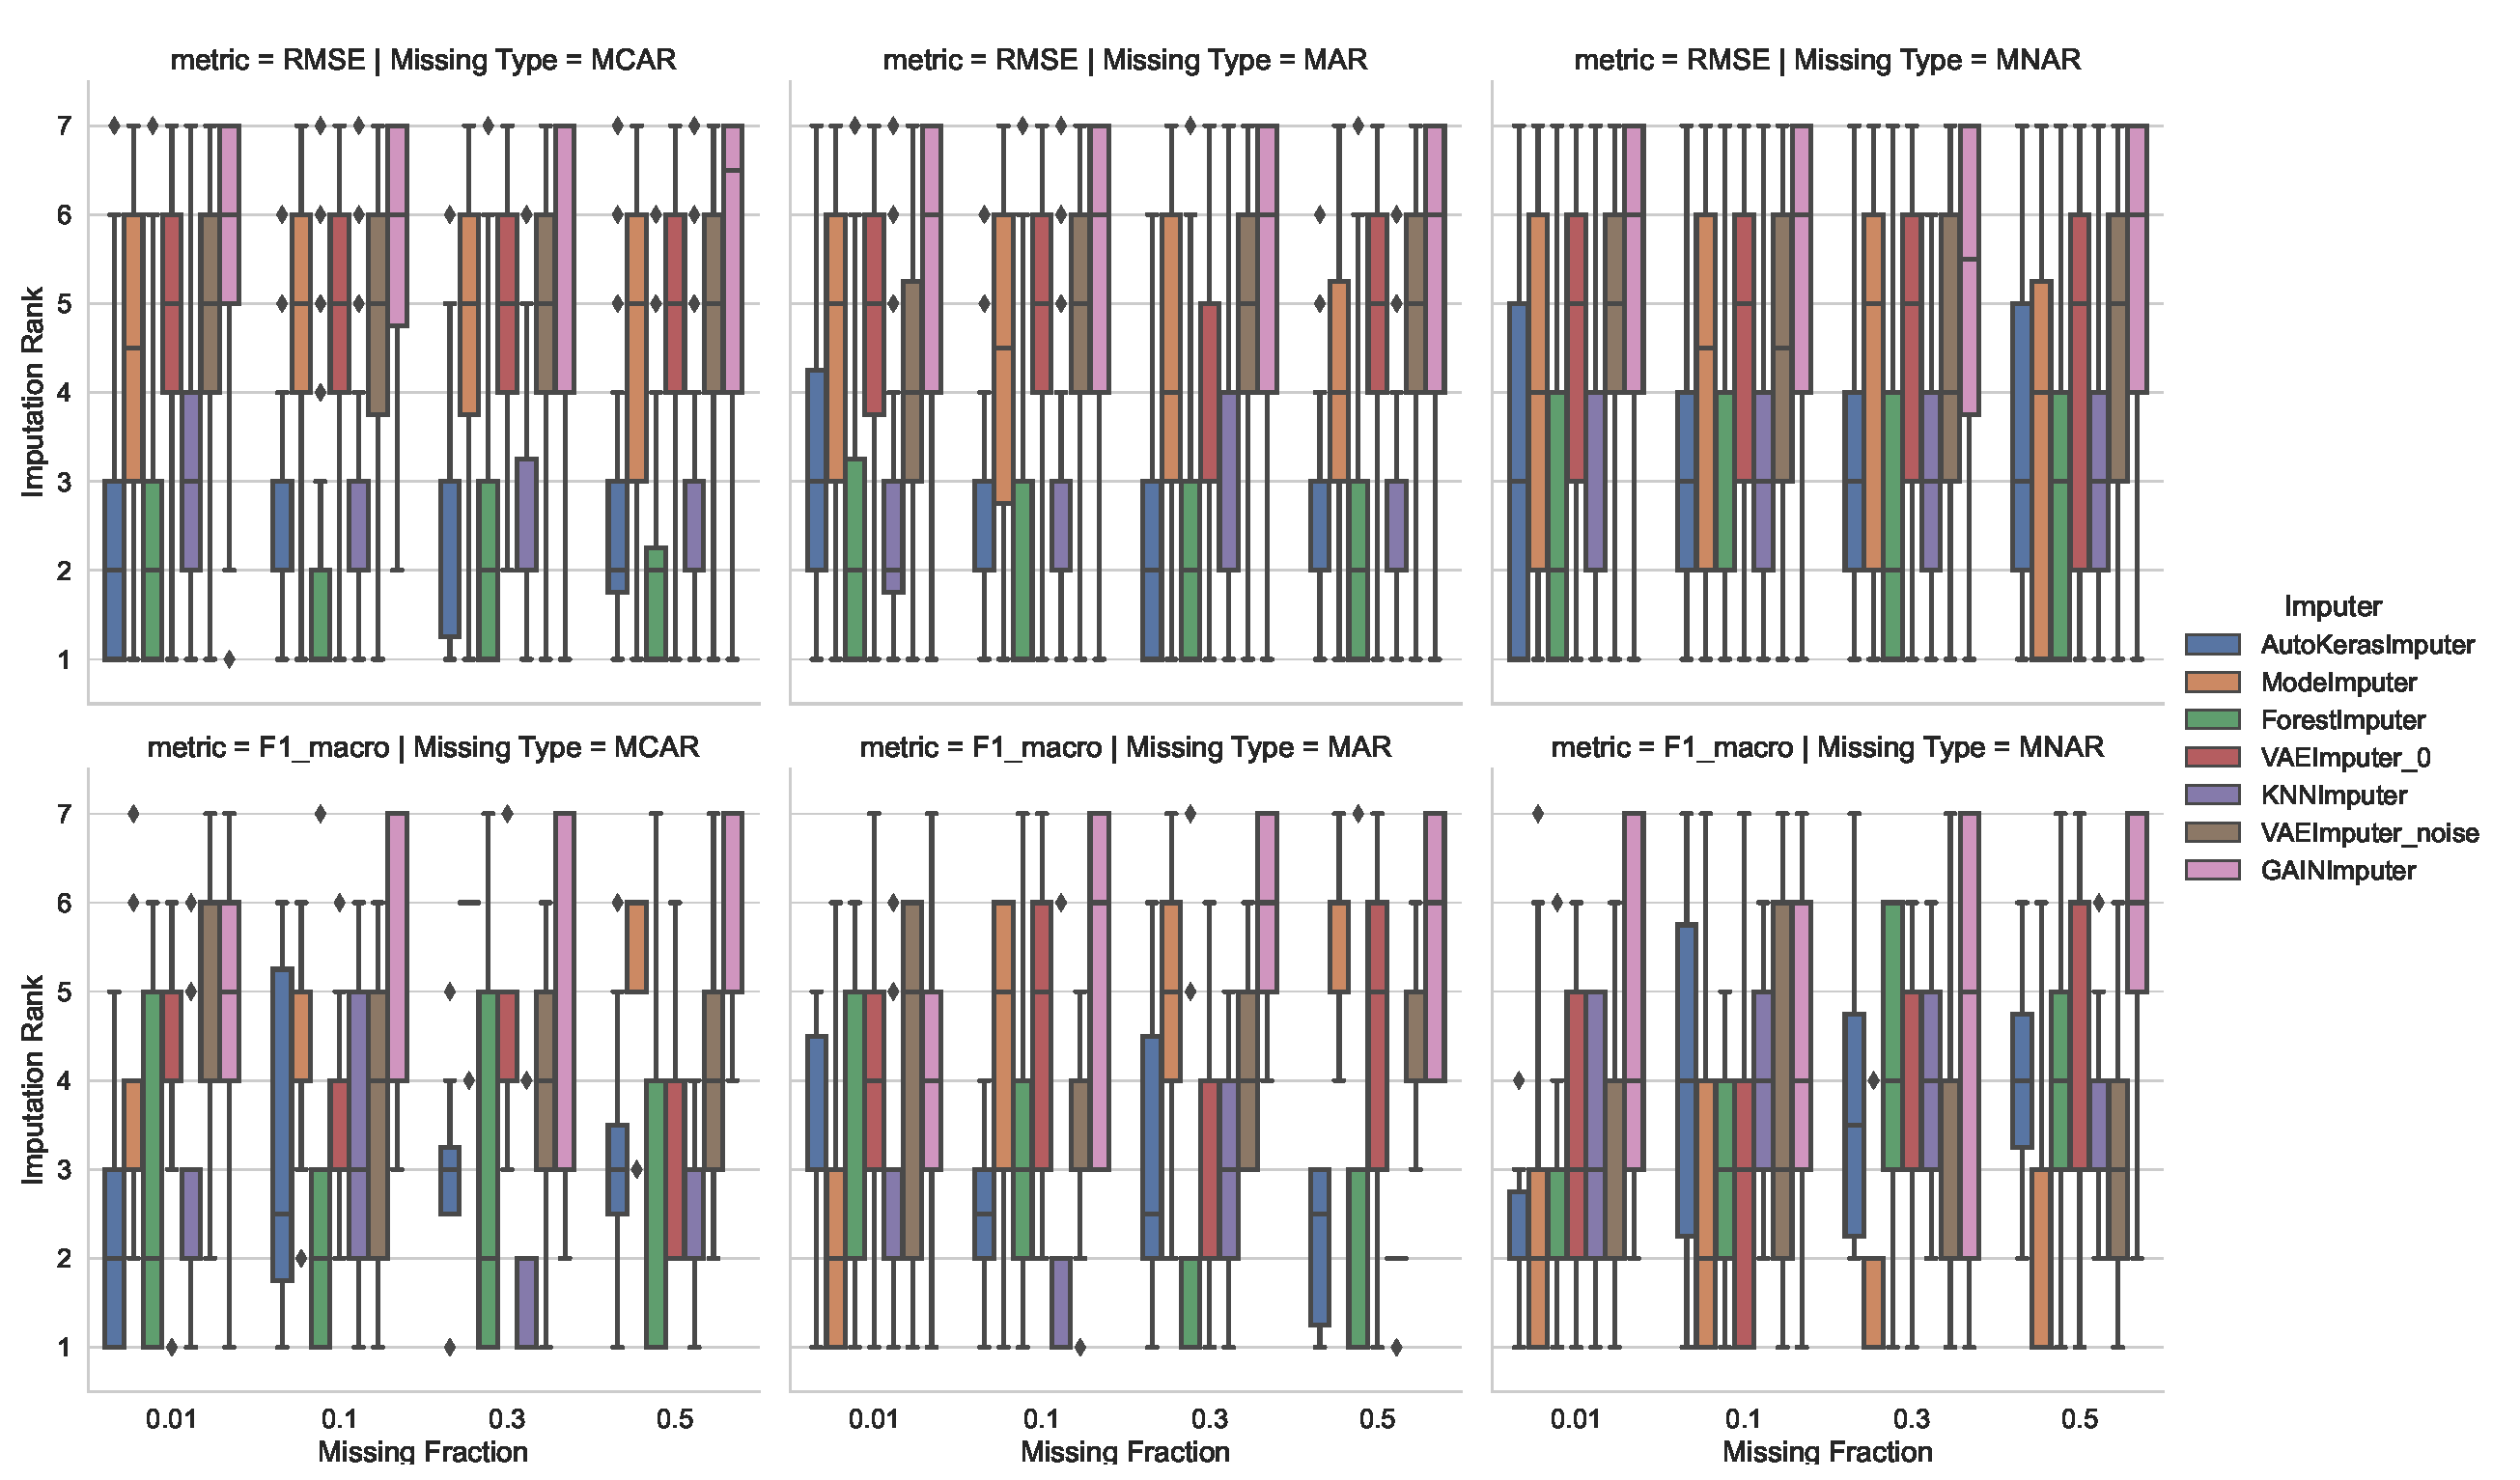
\includegraphics[width=1\columnwidth]{corrupted_impute_rank_boxplot.eps}

    \caption[Scenario 2 Imputation Ranks]{In this figure, we visualize the results of \textit{Experiment 1} (imputation quality) in the \textit{Scenario 2} setting. The imputation rank is plotted against the missingness fraction. The plot is divided into six sub-plots, with three columns determined by the missingness type, ordered by task difficulty from easiest to hardest (MCAR, MAR, MNAR). In the first row of sub-plots we depict results of regression tasks, whereas the second row contains classification results. Within a single sub-plot, each box represents the distibution of ranks of a single imputer over all corresponding datasets/columns.
        \felix{we could strip the imputer from each method and save some space, also fonts should not be cut in the bottom of the figure (call tight layout at the end of the plotting) and we should squeeze the height a bit more}
    }\label{fig:corrupted_impute_rank_boxplot}
\end{figure}

In Figure \ref{fig:corrupted_impute_rank_boxplot} we observe the following effects ...
TODO
